%% Finance Research Letters submission draft (extended)
%% Compile: pdflatex frl_position (twice)
%% Numbers from Analysis/scripts/{t9_main_regressions,frl_capability_pricing}.R
%% Companion full-length paper: gfj_main.tex (formation + measurement audit)
%%
%% HIGHLIGHTS (submit as separate file):
%% - We study 124 day-verified LLM releases and 101 index-member firms, 2022-2026
%% - Model capability scores carry no positive price; closed-source slope is negative
%% - Upstream hardware and rival developers earn 1.6-1.7pp abnormal returns
%% - Firms deploying AI in conventional businesses show precisely zero response
%% - Capability matters only as an amplifier of supply-chain position

\documentclass[review,12pt,authoryear]{elsarticle}

\usepackage{amsmath,amssymb}
\usepackage{booktabs}
\usepackage{graphicx}
\usepackage{threeparttable}
\graphicspath{{figures/}}

\newcommand{\pp}{\,pp}
\journal{Finance Research Letters}

\begin{document}

\begin{frontmatter}

\title{Position, Not Capability:\\How Stock Markets Price Large Language Model Releases}

\author[sdu]{Zhuo Chen\corref{cor1}}
\ead{zhuochen@sdu.edu.cn}
\author[sdu]{Ruishuang Lu}
\cortext[cor1]{Corresponding author.}
\affiliation[sdu]{organization={Center for Economic Research, Shandong University},
city={Jinan}, country={China}}

\begin{abstract}
Do stock markets price the capability of large language models, or the
economic position of firms around a release? Using 124 day-verified model
releases (2022--2026), benchmark capability scores, and double-blind-coded
ecosystem positions for Nasdaq-100 firms, we find capability is not
positively priced: the slope is zero pooled, significantly negative among
closed-source flagships, and zero among unrelated firms. Position is priced:
hardware suppliers and rival developers earn 1.6--1.7 percentage points over
twenty days, with immediate abnormal volume, while firms deploying AI in
conventional businesses show precisely zero price and volume response.
Capability matters only as an amplifier of the hardware premium.
\end{abstract}

\begin{keyword}
Large language models \sep Event study \sep Capability pricing \sep
AI supply chain \sep Abnormal volume
\\ \textit{JEL codes}: G14 \sep O33 \sep G12
\end{keyword}

\end{frontmatter}

%% ============================================================
\section{Introduction}
%% ============================================================

Large language model (LLM) releases have become routine, salient information
events---124 benchmark-qualified releases in our 2022--2026 sample, roughly
one per week by the sample's end. Each arrives with a scorecard: third-party
evaluators publish standardized capability indices within days, and
financial commentary routinely reads those scores as value-relevant news. A
natural hypothesis, implicit in exposure-based studies of AI and asset
prices \citep{eisfeldt2023,babina2024}, is that markets reward measured
capability: the more capable the model, the larger the revaluation of
exposed firms. The hypothesis has intuitive appeal---capability is the
technological object a release delivers---and it underlies both scorecard
journalism and the growing practice of ranking firms by AI exposure.

This letter tests the capability hypothesis directly and rejects it. Across
87 language-model releases with capability scores, the cross-sectional slope
of announcement returns on capability is zero. Where theory says capability
rents should be steepest---closed-source releases, whose developers can
appropriate capability through API pricing and ecosystem lock-in
\citep{teece1986}---the slope is significantly \emph{negative}. What markets
price instead, consistently and increasingly, is \emph{where a firm sits} in
the AI production chain: suppliers of compute inputs and rival model
developers revalue on release, firms that merely use AI do not, and
capability matters only by scaling the compute suppliers' premium.

Our design combines three measurement inputs that are, to our knowledge, new
in combination. First, release dates verified to the day against first-party
sources---vendor engineering blogs, release notes, model repositories, and
archived first captures---for every event; secondary aggregators, we find,
misdate a substantial share of releases, sometimes by months, and misdated
events mechanically decouple returns from announcements. Second, a direct
measure of model capability: the Artificial Analysis intelligence index, a
composite of standardized reasoning and knowledge benchmarks published by a
third-party evaluator, rather than a text- or investment-based proxy. Third,
ecosystem positions assigned to each (firm, developer) pair by two
independent coders under a fixed eight-dimension codebook---hardware
supplier, cloud platform, integrator, deployer, enabler, competitor,
investor, owner---with 99.0\% cell-level agreement and dimension-level
Cohen's $\kappa$ between 0.84 and 1.00. The firm universe is the Nasdaq-100,
so selection into the sample is exogenous to any AI hypothesis, and the
thirty-one constituents with no classifiable AI relationship (consumer
staples, utilities, health care) supply a within-event control group.

Three results follow. First, capability is not positively priced. The pooled
slope of twenty-day cumulative abnormal returns (CARs) on capability is
$-0.01$\pp{} per index point ($p=0.51$). Among the fifty closed-source
releases the slope is $-0.06$\pp{} per point---about $-0.8$\pp{} per
standard deviation of capability ($p=0.024$), and $-1.3$\pp{} per standard
deviation under a three-factor benchmark ($p<0.001$). Among firms with no
ecosystem relationship the slope is an exact zero ($p=0.80$), as a placebo
requires. The negative flagship slope is an anticipation gradient rather
than a penalty on capability: the most capable releases are the most rumored
and scheduled, so their information reaches prices before the announcement
window, and the highest-scoring closed releases in the sample all carry
\emph{positive} average CARs. Second, position is priced. Hardware suppliers
earn 1.66\pp{} and rival developers 1.61\pp{} over $[0,+20]$
($p\approx0.01$), with abnormal trading volume on the announcement day
itself; deployers---firms using AI inside conventional businesses---show a
CAR of $-0.07$\pp{} with a standard error of 0.25\pp{} and no abnormal
volume at any horizon: a genuine zero, not offsetting disagreement. Third,
the two dimensions interact exactly as derived-demand logic implies:
capability carries no average price, but each standard deviation of
capability adds roughly 1.3\pp{} to the hardware premium (interaction
$p=0.088$). A more capable model is bigger news for compute suppliers---not
for the average ``exposed'' firm.

The letter's contribution is to unbundle ``AI exposure.'' Exposure rankings,
whether based on labor-task text measures or investment intensity, conflate
firms on opposite sides of the same shock: a chip designer, a cloud
platform, and a software deployer are all ``highly exposed,'' yet their
announcement returns differ by economically large margins and even in the
sign of the trading response. Once positions are separated, the pricing
loads on the compute-complementarity channel and on positive industry
spillovers to rivals---the contagion pattern of \citet{lang1992} rather than
the competitive-displacement pattern documented for conventional product
introductions \citep{chen2005}---while the displacement channel that
dominates public commentary is priced at a precise zero. A companion
full-length paper documents \emph{when} this pricing rule formed (it is a
2025 phenomenon, coinciding with the reasoning paradigm's shift of compute
demand toward inference) and reports a forensic measurement audit in which
two opposite headline results from an earlier, hand-collected vintage of the
data prove to be artifacts of misdated events and contaminated return
windows. Here we hold the reproducible pipeline fixed and focus on the
cross-sectional question: capability or position.

Section~\ref{sec:data} describes the data. Section~\ref{sec:results}
presents the capability tests, the position premia, and the volume evidence.
Section~\ref{sec:robust} summarizes robustness. Section~\ref{sec:conclusion}
concludes.

%% ============================================================
\section{Data}\label{sec:data}
%% ============================================================

\subsection{Events and dates}

The event universe intersects two independent public sources: the AI
Timeline chronology of model releases and Artificial Analysis (AA) benchmark
coverage. Requiring AA coverage screens out announcements too minor to be
benchmarked; identity matching between the sources is resolved by a scored
matcher with every manual decision recorded in an auditable table, and
same-day family announcements are merged into single events. Of 134
candidate events, 125 have day-level dates verified against first-party
evidence and 124 enter the main sample (one event is excluded because its
identity is inconsistent across sources): 3 events from 2022, 8 from 2023,
45 from 2024, 59 from 2025, and 9 from 2026. Eighty-seven are language-model
releases with AA intelligence scores; thirty-five are media-generation
releases; forty-seven release open weights; forty-one are reasoning models.

Two dating pitfalls deserve note because they generalize to any AI event
study. Vendor content systems sometimes render timestamps in UTC, shifting a
U.S. afternoon announcement to the next calendar day; and Chinese
developers' pages carry Beijing dates, which typically coincide with the
correct U.S. reaction day rather than requiring adjustment. We additionally
recover intraday release times for 55 events from page metadata and archived
first captures; only two events show positive evidence of after-hours
release, and Section~\ref{sec:robust} confirms that no feasible re-dating
changes the results.

\subsection{Positions, capability, and outcomes}

Each of the $108\times25$ (firm, developer) pairs is coded on eight
dimensions under a fixed codebook by two independent coders; disagreements
(1.0\% of cells) were adjudicated against the codebook with all decisions
logged. Event-level indicators take the union across the event's developers.
In the main Nasdaq-100 sample, 25\% of firm-events carry a hardware
relationship, 5\% cloud, 12\% integrator, 20\% deployer, and 5\% competitor;
26\% belong to control firms with no relationship on any dimension.
Capability is the AA intelligence index of the event's flagship model (the
highest-scoring variant; sample standard deviation 12.7). Because the index
is a composite over standardized benchmarks, it is comparable across
developers at a point in time---precisely the comparison our within-year
specifications exploit.

Daily total returns come from adjusted closes (January 2021 to April 2026).
Market-model CARs use the S\&P~500 as market proxy with estimation window
$[-200,-10]$ (minimum 120 observations), cumulated over $[0,+w]$ for
$w\le20$ and a pre-event window $[-10,-2]$; we deliberately avoid a
Nasdaq-100 benchmark because sample firms are its constituents, and we
compute three-factor CARs for robustness. Abnormal volume is the deviation
of daily log volume from its estimation-window mean, in estimation-window
standard deviations, averaged over the event window. Firm controls (log
assets, book-to-market with a negative-equity flag, momentum, volatility)
are matched under a strict 45-day as-of rule so that only statements
publicly available at the event enter. Standard errors are clustered by
event (CR2) throughout; event-fixed-effects specifications identify from
within-event variation alone.

%% ============================================================
\section{Results}\label{sec:results}
%% ============================================================

\subsection{Capability is not priced}

Table~\ref{tab:capability} regresses CAR$[0,+20]$ on capability with firm
controls and year fixed effects, so the slope compares releases within the
same year---not GPT-4 against successors three benchmark generations later.
Column (1): the pooled slope is $-0.0001$ per index point ($p=0.51$).
Column (2) restricts to the fifty closed-source releases, where
appropriability logic predicts the steepest capability rents; the slope is
$-0.0006$ ($p=0.024$). Column (3): among the thirty-seven open-weight
releases the slope is 0.0000 ($p=0.93$). Column (4) is the placebo: among
firms with no ecosystem relationship the slope is $-0.0001$ ($p=0.80$).
Capability scores do not predict returns where no economic channel exists,
so the closed-source negative is not a mechanical artifact of the score
itself.

\begin{table}[t!]
\centering
\begin{threeparttable}
\caption{Model capability and abnormal returns}\label{tab:capability}
\small
\begin{tabular}{lccccc}
\toprule
 & (1) All & (2) Closed & (3) Open & (4) Placebo & (5) Interaction \\
 &  &  &  & (unrelated firms) &  \\
\midrule
AA intelligence     & $-$0.0001 & $-$0.0006** & 0.0000 & $-$0.0001 & $-$0.0003 \\
                    & (0.0002) & (0.0002) & (0.0003) & (0.0004) & (0.0002) \\
$\times$ Upstream hardware & & & & & 0.0010* \\
                    & & & & & (0.0006) \\
Upstream hardware   & & & & & 0.0207*** \\
                    & & & & & (0.0078) \\
\midrule
Events              & 87 & 50 & 37 & 87 & 87 \\
Observations        & 8{,}562 & 4{,}917 & 3{,}645 & 2{,}784 & 8{,}562 \\
\bottomrule
\end{tabular}
\begin{tablenotes}\footnotesize
\item Notes: Dependent variable is the market-model CAR$[0,+20]$. All columns
include firm controls (log assets, book-to-market with negative-equity flag,
volatility, momentum) and year fixed effects; capability is centered in
column (5). Standard errors clustered by event (CR2). *, **, *** denote
10\%, 5\%, 1\%.
\end{tablenotes}
\end{threeparttable}
\end{table}

The negative closed-source slope has a natural reading: anticipation. Within
a year, the most capable releases are flagship events, rumored for months
and often pre-announced to the day, while lower-scoring releases arrive with
less warning and deliver larger surprises. Three facts support this reading.
The eight highest-scoring closed releases in the sample all carry positive
average CARs of $+0.1$ to $+2.9$\%---flagships are not punished; they are
pre-priced. The negative slope concentrates in the later sample ($-0.0006$,
$p=0.04$, in 2025--2026 against $-0.0001$, $p=0.87$, in 2022--2024), when
release calendars became crowded and heavily previewed. And replacing the
level with a surprise measure---the score's distance above the pre-event
frontier maximum---yields the same pattern, because benchmark-measured
surprise still correlates with exactly the flagship status that markets
anticipate; separating true expectation errors from levels would require
ex-ante forecast data that do not yet exist for model benchmarks.

Column (5) shows what capability \emph{does} do: interacted with the
hardware indicator (capability centered), each index point adds 0.10\pp{} to
the hardware premium ($p=0.088$)---roughly 1.3\pp{} per standard
deviation---while the hardware main effect at mean capability is 2.07\pp{}
($p=0.010$). Capability is priced as a scaling factor on derived compute
demand, not as a stand-alone characteristic.

\subsection{Position is priced}

Table~\ref{tab:position} turns to positions. Hardware suppliers earn
1.66\pp{} more than unrelated constituents over the twenty days after a
release ($p=0.012$); the estimate is 1.79\pp{} under the three-factor
benchmark and 1.54\pp{} with event fixed effects, where identification comes
only from within-event comparisons of firms facing the same release, the
same market conditions, and the same AI sentiment. Rival model
developers---listed firms that develop competing frontier models---earn a
statistically indistinguishable 1.61\pp{}. The positive competitor spillover
is itself informative: product-introduction studies typically find negative
wealth effects for rivals \citep{chen2005}; the positive sign indicates that
in this period a release conveyed industry-level growth information that
dominated competitive displacement, the contagion pattern of
\citet{lang1992} in a fast-expanding technology sector.

\begin{table}[t!]
\centering
\begin{threeparttable}
\caption{Ecosystem position and abnormal returns}\label{tab:position}
\small
\begin{tabular}{lccc}
\toprule
Dependent variable: & (1) CAR$^{MM}[0,20]$ & (2) CAR$^{FF3}[0,20]$ & (3) CAR$^{MM}[0,20]$ \\
\midrule
Upstream hardware      & 0.0166** & 0.0179*** & 0.0154** \\
                       & (0.0065) & (0.0065)  & (0.0066) \\
Upstream cloud         & $-$0.0011 & 0.0020   & $-$0.0018 \\
                       & (0.0078) & (0.0074)  & (0.0076) \\
Downstream integrator  & $-$0.0051 & $-$0.0041 & $-$0.0053 \\
                       & (0.0049) & (0.0048)  & (0.0050) \\
Downstream deployer    & $-$0.0007 & 0.0002   & $-$0.0011 \\
                       & (0.0025) & (0.0024)  & (0.0025) \\
Competitor             & 0.0161** & 0.0159*** & 0.0158** \\
                       & (0.0064) & (0.0058)  & (0.0064) \\
\midrule
Investor, owner        & Yes & Yes & Yes \\
Firm controls          & Yes & Yes & Yes \\
Year fixed effects     & Yes & Yes & --- \\
Event fixed effects    & --- & --- & Yes \\
Observations           & 12{,}112 & 12{,}112 & 12{,}112 \\
Events                 & 124 & 124 & 124 \\
\bottomrule
\end{tabular}
\begin{tablenotes}\footnotesize
\item Notes: Investor and owner/publisher indicators included (positive,
insignificant; their positive cells concentrate in few developers, hence few
clusters). Standard errors clustered by event (CR2). *, **, *** denote
10\%, 5\%, 1\%.
\end{tablenotes}
\end{threeparttable}
\end{table}

The deployer coefficient is $-0.07$\pp{} with a standard error of 0.25\pp{}.
This is not an underpowered non-result: the 95\% confidence interval,
$[-0.56,+0.42]$\pp{}, excludes deployer losses larger than one third of the
hardware gain. Whatever the long-run effects of foundation models on
downstream businesses, four years of release events contain no evidence that
markets price displacement on announcement. The remaining positions sharpen
the picture. Cloud platforms---the most direct resellers of model
capability---show a price response of zero ($-0.11$\pp{}, $p=0.89$), a fact
whose meaning emerges from the volume evidence below. Integrators are mildly
negative and imprecise ($-0.51$\pp{}, $p=0.30$). The economically meaningful
contrast is the roughly 1.7\pp{} spread between hardware and deployers
within the same event window---firms distinguished only by where they sit in
the production chain.

The premium is not a single-stock story. Dropping any one hardware firm
leaves the coefficient between 1.2 and 1.6\pp{} across twenty-three
leave-one-out fits; excluding NVIDIA specifically gives 1.5\pp{}
($p=0.023$); and hardware members outside the semiconductor index proper
(server, networking, and storage suppliers) earn at least as much as
semiconductor names. Nor is it a level effect of the AI era: at the
portfolio level, a calendar-time strategy long the hardware suppliers and
short the downstream firms earns a three-factor alpha of roughly 24\%
annualized over the sample ($p=0.054$), though with release windows covering
56\% of trading days we read the portfolio as economic scale rather than
identification, which rests on the within-event estimates.

Figure~\ref{fig:profile} traces the accumulation. In the full sample the
hardware premium is invisible at the close of the announcement day, emerges
by $[0,+10]$ (0.98\pp{}, $p=0.02$), and reaches 1.66\pp{} by day twenty; in
the 2025--2026 subsample---after the pricing rule strengthened, as the
companion paper documents---it is significant from $[0,+2]$ ($+0.51$\pp{})
and accumulates monotonically to 4.28\pp{}. The deployer line never leaves
zero at any horizon. Two checks address the concern that slow accumulation
reflects confounded drift: controlling for each firm's own pre-event CAR
leaves the post-event estimates essentially unchanged (4.28 to 4.35\pp{} in
the late sample), and the pre-event hardware run-up that does exist
($+1.4$\pp{} over $[-10,-2]$ in 2025--2026) is not accompanied by any
abnormal volume, consistent with thin pre-announcement positioning rather
than information leakage.

\begin{figure}[t!]
\centering
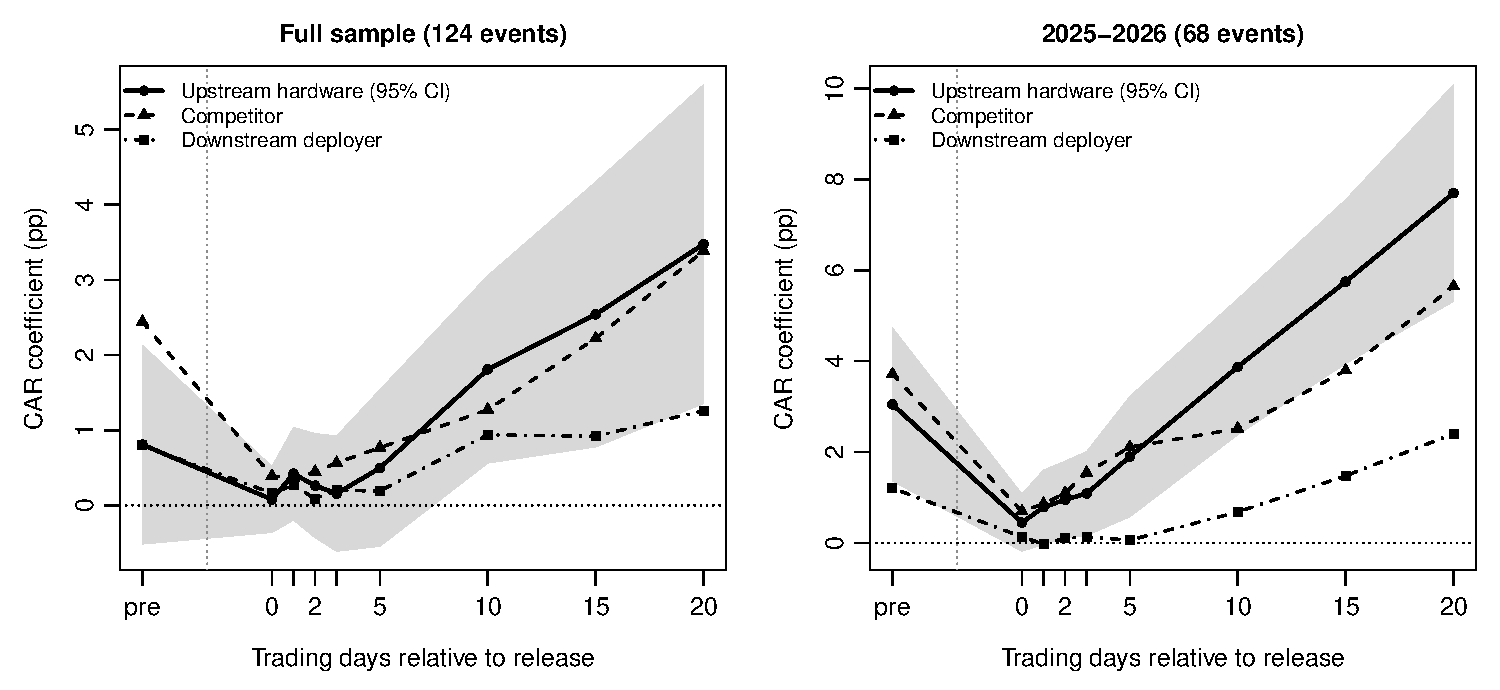
\includegraphics[width=\textwidth]{fig1_car_profile}
\caption{Cumulative abnormal returns by ecosystem position and accumulation
window. Coefficients from window-by-window cross-sectional regressions with
firm controls and year fixed effects; shading is the 95\% band for the
hardware coefficient (CR2, clustered by event). The leftmost point is the
pre-event window $[-10,-2]$. Left panel: full sample; right panel:
2025--2026.}
\label{fig:profile}
\end{figure}

\subsection{Volume separates attention, disagreement, and irrelevance}

Abnormal volume completes the taxonomy (Table~\ref{tab:volume}), and it is
where the three downstream fates separate most cleanly. Hardware suppliers
trade 0.12 standard deviations above normal on the announcement day
($p<0.001$)---including in the full sample, where the same-horizon price
response is still indistinguishable from zero. Attention arrives
immediately; directional consensus takes days to form. That
sequencing---volume first, price later---is the signature of gradual
information incorporation rather than of a return drift unrelated to the
event.

Deployers show no abnormal volume at any horizon ($p=0.74$ at $[0,+1]$).
Combined with the precise price zero, this rules out the interpretation that
deployer investors disagree and net out: there is simply nothing to trade.
Cloud platforms are the mirror image and the most striking cell in the
panel: abnormal volume of 0.29 standard deviations at $[0,+1]$ (0.44 in
2025--2026), already 0.20 standard deviations in the \emph{pre-event}
window, and yet a price response of zero throughout. In disagreement models,
volume without price movement is the fingerprint of investors interpreting
the same public signal with opposite priors \citep{kandel1995}. Cloud
platforms fit naturally: a frontier release is simultaneously good news for
their compute-rental business and bad news for their own model ambitions and
gross margins, and the market splits on the net. The taxonomy, then:
hardware is priced with consensus, cloud is traded without consensus, and
deployers are ignored on both margins.

\begin{table}[t!]
\centering
\begin{threeparttable}
\caption{Abnormal trading volume}\label{tab:volume}
\small
\begin{tabular}{lcc@{\hskip 2em}cc}
\toprule
 & \multicolumn{2}{c}{Full sample} & \multicolumn{2}{c}{2025--2026} \\
\cmidrule(lr){2-3}\cmidrule(l){4-5}
Window: & $[-10,-2]$ & $[0,+1]$ & $[-10,-2]$ & $[0,+1]$ \\
\midrule
Upstream hardware   & 0.033 & 0.121*** & 0.046 & 0.106*** \\
                    & (0.026) & (0.036) & (0.032) & (0.036) \\
Upstream cloud      & 0.204*** & 0.292*** & 0.314*** & 0.435*** \\
                    & (0.041) & (0.049) & (0.046) & (0.063) \\
Downstream deployer & $-$0.019 & 0.006 & 0.024 & 0.028 \\
                    & (0.015) & (0.019) & (0.018) & (0.021) \\
Competitor          & $-$0.037 & $-$0.017 & $-$0.014 & $-$0.081 \\
                    & (0.029) & (0.043) & (0.041) & (0.052) \\
\midrule
Event fixed effects & Yes & Yes & Yes & Yes \\
\bottomrule
\end{tabular}
\begin{tablenotes}\footnotesize
\item Notes: Standardized abnormal log volume (deviation from the
$[-200,-10]$ mean in estimation-window SDs, averaged over the window). Firm
controls included; SEs clustered by event (CR2). *, **, *** denote 10\%,
5\%, 1\%.
\end{tablenotes}
\end{threeparttable}
\end{table}

%% ============================================================
\section{Robustness}\label{sec:robust}
%% ============================================================

The position premia are significant in 16--17 of 20 specifications spanning
benchmark models (S\&P~500, Nasdaq-100, SOX, three-factor), accumulation
windows ($[0,10]$, $[0,15]$), winsorization at 1\%/99\%, restriction to
high-confidence dates, exclusion of the six multi-component events, event
fixed effects, and a pre-event CAR control; the deployer zero and the null
hardware~$\times$~open-weight interaction ($p=0.90$) hold in all twenty. The
open-weight null deserves emphasis given the public narrative that efficient
open models threaten compute rents: releases that publish weights generate
the same hardware premium as proprietary ones. Event-day conventions do not
matter: announcement timestamps recovered for 55 events identify only two
after-hours releases, and shifting \emph{every} event by one trading day
leaves the late-sample hardware estimate at 4.7\pp{} ($p<0.001$). The
capability results are likewise insensitive to three-factor benchmarks, to
the surprise transformation, and to restricting the sample to firms with any
AI relationship; and an independent 3,144-specification search over
outcomes, samples, moderators, and fixed-effect structures finds the
hardware--time interaction positive in 100\% of specifications (family-wise
$q=0.002$).

%% ============================================================
\section{Conclusion}\label{sec:conclusion}
%% ============================================================

Around LLM releases, equity markets do not pay for capability---they pay for
position. Benchmark scores carry no positive premium, and a negative one
among the anticipated flagships where capability rents should be steepest;
hardware suppliers and rival developers revalue by 1.6--1.7\pp{} per release
while AI-deploying firms show precisely zero price and volume response; and
capability enters pricing only by scaling the hardware premium. The volume
evidence adds a taxonomy that returns alone cannot deliver: consensus
pricing upstream, unresolved disagreement at cloud platforms, and genuine
irrelevance downstream.

The results carry two lessons. For research that ranks firms by AI exposure,
exposure conflates positions with opposite pricing; the economically active
margin is the supply-chain role, and pooling roles attenuates estimated AI
effects toward zero. For the public debate, four years of high-frequency
technology news contain no evidence that markets price AI displacement of
downstream businesses on announcement---the displacement narrative, whatever
its long-run merit, is not in prices. A natural extension is expectations
data: analyst reports and earnings-call language can date when
compute-demand reasoning entered the sell-side lexicon and test the
anticipation mechanism we infer from the flagship gradient directly.

%% ============================================================
\section*{Data availability}
The event pipeline, coding decision tables, and estimation code are
available from the authors.

%% ============================================================
\begin{thebibliography}{00}
\expandafter\ifx\csname natexlab\endcsname\relax\def\natexlab#1{#1}\fi

\bibitem[Babina et al.(2024)]{babina2024}
Babina, T., Fedyk, A., He, A., Hodson, J., 2024. Artificial intelligence,
firm growth, and product innovation. Journal of Financial Economics 151,
103745.

\bibitem[Chen et al.(2005)]{chen2005}
Chen, S.-S., Ho, K.~W., Ik, K.~H., 2005. The wealth effect of new product
introductions on industry rivals. Journal of Business 78, 969--996.

\bibitem[Eisfeldt et al.(2023)]{eisfeldt2023}
Eisfeldt, A.~L., Schubert, G., Zhang, M.~B., 2023. Generative AI and firm
values. NBER Working Paper 31222.

\bibitem[Kandel and Pearson(1995)]{kandel1995}
Kandel, E., Pearson, N.~D., 1995. Differential interpretation of public
signals and trade in speculative markets. Journal of Political Economy 103,
831--872.

\bibitem[Lang and Stulz(1992)]{lang1992}
Lang, L.~H.~P., Stulz, R.~M., 1992. Contagion and competitive intra-industry
effects of bankruptcy announcements. Journal of Financial Economics 32,
45--60.

\bibitem[Teece(1986)]{teece1986}
Teece, D.~J., 1986. Profiting from technological innovation: Implications
for integration, collaboration, licensing and public policy. Research Policy
15, 285--305.

\end{thebibliography}

\end{document}
